\documentclass{standalone}
\usepackage{tikz}
\usetikzlibrary{patterns, positioning}


\begin{document}
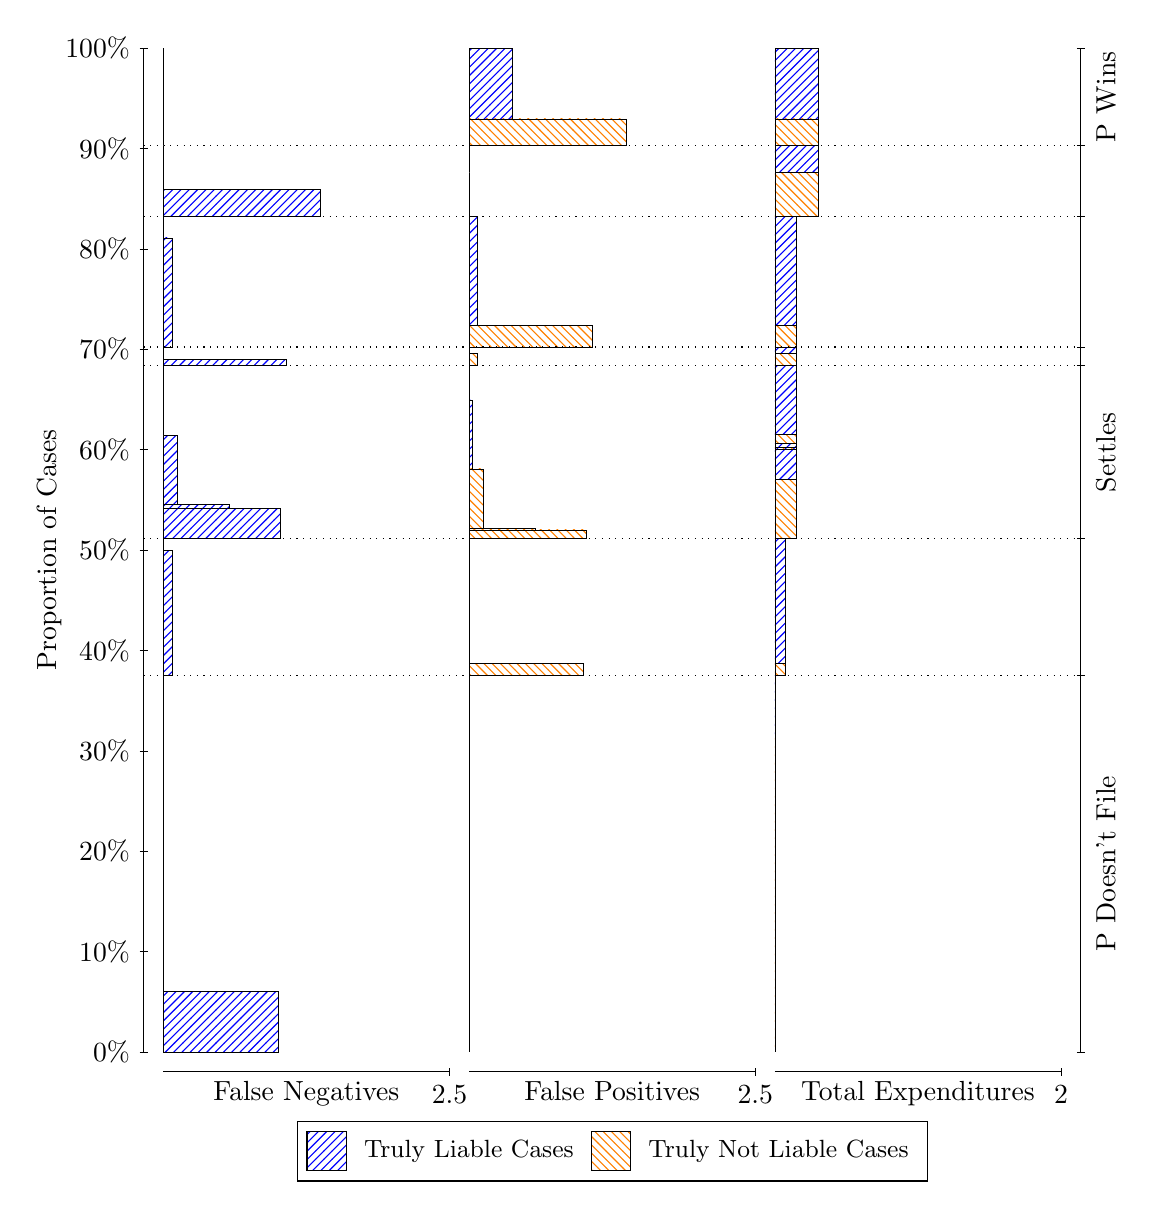
\begin{tikzpicture}
\draw[black, very thin] (1.5,1.75) -- (1.5,14.5);
\node[rotate=90, text=black, anchor=center] at (0.3, 8.125) {Proportion of Cases};
\draw[black, very thin] (1.45,1.75) -- (1.55,1.75);
\node[text=black, anchor=east] at (1.45, 1.75) {0\%};
\draw[black, very thin] (1.45,3.025) -- (1.55,3.025);
\node[text=black, anchor=east] at (1.45, 3.025) {10\%};
\draw[black, very thin] (1.45,4.3) -- (1.55,4.3);
\node[text=black, anchor=east] at (1.45, 4.3) {20\%};
\draw[black, very thin] (1.45,5.575) -- (1.55,5.575);
\node[text=black, anchor=east] at (1.45, 5.575) {30\%};
\draw[black, very thin] (1.45,6.85) -- (1.55,6.85);
\node[text=black, anchor=east] at (1.45, 6.85) {40\%};
\draw[black, very thin] (1.45,8.125) -- (1.55,8.125);
\node[text=black, anchor=east] at (1.45, 8.125) {50\%};
\draw[black, very thin] (1.45,9.4) -- (1.55,9.4);
\node[text=black, anchor=east] at (1.45, 9.4) {60\%};
\draw[black, very thin] (1.45,10.675) -- (1.55,10.675);
\node[text=black, anchor=east] at (1.45, 10.675) {70\%};
\draw[black, very thin] (1.45,11.95) -- (1.55,11.95);
\node[text=black, anchor=east] at (1.45, 11.95) {80\%};
\draw[black, very thin] (1.45,13.225) -- (1.55,13.225);
\node[text=black, anchor=east] at (1.45, 13.225) {90\%};
\draw[black, very thin] (1.45,14.5) -- (1.55,14.5);
\node[text=black, anchor=east] at (1.45, 14.5) {100\%};

\draw[black, very thin] (13.4,1.75) -- (13.4,14.5);
\draw[black, very thin] (13.35,1.75) -- (13.45,1.75);
\node[anchor=west] at (13.35, 1.75) {};
\draw[black, very thin] (13.35,6.5344) -- (13.45,6.5344);
\node[anchor=west] at (13.35, 6.5344) {};
\draw[black, very thin] (13.35,8.268) -- (13.45,8.268);
\node[anchor=west] at (13.35, 8.268) {};
\draw[black, very thin] (13.35,10.467) -- (13.45,10.467);
\node[anchor=west] at (13.35, 10.467) {};
\draw[black, very thin] (13.35,10.703) -- (13.45,10.703);
\node[anchor=west] at (13.35, 10.703) {};
\draw[black, very thin] (13.35,12.365) -- (13.45,12.365);
\node[anchor=west] at (13.35, 12.365) {};
\draw[black, very thin] (13.35,13.259) -- (13.45,13.259);
\node[anchor=west] at (13.35, 13.259) {};
\draw[black, very thin] (13.35,14.5) -- (13.45,14.5);
\node[anchor=west] at (13.35, 14.5) {};

\draw[black, very thin, pattern color=blue, pattern=north east lines] (1.75,1.75) rectangle (3.2033,2.5199);
\draw[black, very thin, pattern color=orange, pattern=north west lines] (1.75,2.5199) rectangle (1.75,6.5344);
\draw[black, very thin, pattern color=blue, pattern=north east lines] (1.75,6.5344) rectangle (1.859,8.1192);
\draw[black, very thin, pattern color=orange, pattern=north west lines] (1.75,8.1192) rectangle (1.75,8.268);
\draw[black, very thin, pattern color=blue, pattern=north east lines] (1.75,8.268) rectangle (3.2397,8.6536);
\draw[black, very thin, pattern color=blue, pattern=north east lines] (1.75,8.6536) rectangle (2.5857,8.7039);
\draw[black, very thin, pattern color=blue, pattern=north east lines] (1.75,8.7039) rectangle (1.9317,9.5801);
\draw[black, very thin, pattern color=orange, pattern=north west lines] (1.75,9.5801) rectangle (1.75,10.467);
\draw[black, very thin, pattern color=blue, pattern=north east lines] (1.75,10.467) rectangle (3.3123,10.547);
\draw[black, very thin, pattern color=orange, pattern=north west lines] (1.75,10.547) rectangle (1.75,10.703);
\draw[black, very thin, pattern color=blue, pattern=north east lines] (1.75,10.703) rectangle (1.859,12.089);
\draw[black, very thin, pattern color=orange, pattern=north west lines] (1.75,12.089) rectangle (1.75,12.365);
\draw[black, very thin, pattern color=blue, pattern=north east lines] (1.75,12.365) rectangle (3.7483,12.706);
\draw[black, very thin, pattern color=orange, pattern=north west lines] (1.75,12.706) rectangle (1.75,13.259);
\draw[black, very thin, pattern color=orange, pattern=north west lines] (1.75,13.259) rectangle (1.75,13.6);
\draw[black, very thin, pattern color=blue, pattern=north east lines] (1.75,13.6) rectangle (1.75,14.5);
\draw[black, very thin, pattern color=orange, pattern=north west lines] (5.6333,1.75) rectangle (5.6333,5.7644);
\draw[black, very thin, pattern color=blue, pattern=north east lines] (5.6333,5.7644) rectangle (5.6333,6.5344);
\draw[black, very thin, pattern color=orange, pattern=north west lines] (5.6333,6.5344) rectangle (7.0867,6.6832);
\draw[black, very thin, pattern color=blue, pattern=north east lines] (5.6333,6.6832) rectangle (5.6333,8.268);
\draw[black, very thin, pattern color=orange, pattern=north west lines] (5.6333,8.268) rectangle (7.123,8.3795);
\draw[black, very thin, pattern color=orange, pattern=north west lines] (5.6333,8.3795) rectangle (6.469,8.3997);
\draw[black, very thin, pattern color=orange, pattern=north west lines] (5.6333,8.3997) rectangle (5.815,9.1548);
\draw[black, very thin, pattern color=blue, pattern=north east lines] (5.6333,9.1548) rectangle (5.6697,10.031);
\draw[black, very thin, pattern color=blue, pattern=north east lines] (5.6333,10.031) rectangle (5.6333,10.467);
\draw[black, very thin, pattern color=orange, pattern=north west lines] (5.6333,10.467) rectangle (5.7423,10.622);
\draw[black, very thin, pattern color=blue, pattern=north east lines] (5.6333,10.622) rectangle (5.6333,10.703);
\draw[black, very thin, pattern color=orange, pattern=north west lines] (5.6333,10.703) rectangle (7.1957,10.979);
\draw[black, very thin, pattern color=blue, pattern=north east lines] (5.6333,10.979) rectangle (5.7423,12.365);
\draw[black, very thin, pattern color=orange, pattern=north west lines] (5.6333,12.365) rectangle (5.6333,12.918);
\draw[black, very thin, pattern color=blue, pattern=north east lines] (5.6333,12.918) rectangle (5.6333,13.259);
\draw[black, very thin, pattern color=orange, pattern=north west lines] (5.6333,13.259) rectangle (7.6317,13.6);
\draw[black, very thin, pattern color=blue, pattern=north east lines] (5.6333,13.6) rectangle (6.1783,14.5);
\draw[black, very thin, pattern color=orange, pattern=north west lines] (9.5167,1.75) rectangle (9.5167,5.7644);
\draw[black, very thin, pattern color=blue, pattern=north east lines] (9.5167,5.7644) rectangle (9.5167,6.5344);
\draw[black, very thin, pattern color=orange, pattern=north west lines] (9.5167,6.5344) rectangle (9.6529,6.6832);
\draw[black, very thin, pattern color=blue, pattern=north east lines] (9.5167,6.6832) rectangle (9.6529,8.268);
\draw[black, very thin, pattern color=orange, pattern=north west lines] (9.5167,8.268) rectangle (9.7892,9.0231);
\draw[black, very thin, pattern color=blue, pattern=north east lines] (9.5167,9.0231) rectangle (9.7892,9.4087);
\draw[black, very thin, pattern color=orange, pattern=north west lines] (9.5167,9.4087) rectangle (9.7892,9.4289);
\draw[black, very thin, pattern color=blue, pattern=north east lines] (9.5167,9.4289) rectangle (9.7892,9.4791);
\draw[black, very thin, pattern color=orange, pattern=north west lines] (9.5167,9.4791) rectangle (9.7892,9.5906);
\draw[black, very thin, pattern color=blue, pattern=north east lines] (9.5167,9.5906) rectangle (9.7892,10.467);
\draw[black, very thin, pattern color=orange, pattern=north west lines] (9.5167,10.467) rectangle (9.7892,10.622);
\draw[black, very thin, pattern color=blue, pattern=north east lines] (9.5167,10.622) rectangle (9.7892,10.703);
\draw[black, very thin, pattern color=orange, pattern=north west lines] (9.5167,10.703) rectangle (9.7892,10.979);
\draw[black, very thin, pattern color=blue, pattern=north east lines] (9.5167,10.979) rectangle (9.7892,12.365);
\draw[black, very thin, pattern color=orange, pattern=north west lines] (9.5167,12.365) rectangle (10.062,12.918);
\draw[black, very thin, pattern color=blue, pattern=north east lines] (9.5167,12.918) rectangle (10.062,13.259);
\draw[black, very thin, pattern color=orange, pattern=north west lines] (9.5167,13.259) rectangle (10.062,13.6);
\draw[black, very thin, pattern color=blue, pattern=north east lines] (9.5167,13.6) rectangle (10.062,14.5);
\draw[black, dotted] (1.5,6.5344) -- (13.4,6.5344);
\draw[black, dotted] (1.5,8.268) -- (13.4,8.268);
\draw[black, dotted] (1.5,10.467) -- (13.4,10.467);
\draw[black, dotted] (1.5,10.703) -- (13.4,10.703);
\draw[black, dotted] (1.5,12.365) -- (13.4,12.365);
\draw[black, dotted] (1.5,13.259) -- (13.4,13.259);
\draw[black, very thin] (1.75,1.5) -- (5.3833,1.5);
\node[text=black, anchor=north] at (3.5667, 1.5) {False Negatives};
\draw[black, very thin] (5.3833,1.45) -- (5.3833,1.55);
\node[text=black, anchor=north] at (5.3833, 1.45) {2.5};

\draw[black, very thin] (5.6333,1.5) -- (9.2667,1.5);
\node[text=black, anchor=north] at (7.45, 1.5) {False Positives};
\draw[black, very thin] (9.2667,1.45) -- (9.2667,1.55);
\node[text=black, anchor=north] at (9.2667, 1.45) {2.5};

\draw[black, very thin] (9.5167,1.5) -- (13.15,1.5);
\node[text=black, anchor=north] at (11.333, 1.5) {Total Expenditures};
\draw[black, very thin] (13.15,1.45) -- (13.15,1.55);
\node[text=black, anchor=north] at (13.15, 1.45) {2};

\node[text=black, centered, rotate=90] at (13.72, 4.1422) {P Doesn't File};

\node[text=black, centered, rotate=90] at (13.72, 9.3674) {Settles};



\node[text=black, centered, rotate=90] at (13.72, 13.879) {P Wins};

\draw (7.449999999999999,1.5) node[draw=none] (baseCoordinate) {};
\begin{scope}[align=center]
        \matrix[scale=0.5, draw=black, below=0.5cm of baseCoordinate, nodes={draw}, column sep=0.1cm]{
            \node[rectangle, draw, minimum width=0.5cm, minimum height=0.5cm, pattern color=blue, pattern=north east lines] {}; &
            \node[draw=none, font=\small, text=black] (B) {Truly Liable Cases}; &
            \node[rectangle, draw, minimum width=0.5cm, minimum height=0.5cm, pattern color=orange, pattern=north west lines] {}; &
            \node[draw=none, font=\small, text=black] (B) {Truly Not Liable Cases}; \\
            };
\end{scope}

\end{tikzpicture}
\end{document}